\section{Branch-and-Bound Optimization}

%\begin{itemize}
%\item Describe the motivation to use the branch-and-bound to approach the efficiency issues (execute all queries are costly)
%\item The idea is to execute the minimum amount of queries.
%\item Describe the heuristic used to determined when evaluate a query
%\item Describe how those heuristic are used in the framework
%\item Describe how we tackle the time issue.  (reordering queries).
%\item Describe the moment  that attribute queries are generated. (at the beginning of the process)
%\item Describe the moment the queries with class clauses are generated. (they are generated when the cardinality of candidates are above a threshold)
%\item Describe how the predictor can increase the efficiency by skipping queries
%\item Describe how we train the classifier. it is done automatically after it converges.
%\end{itemize}

With the learned key pairs $U^{*st}_A$, now we discuss how to efficiently generate candidate sets by searching for instances that match these keys. We need to retrieve target instances for each of the $n$ source instances. For this, a naive solution would generate $q$ different types of candidate selection queries for every pair of comparable keys. Given $k$ key pairs, it thus would need $n \times k \times q$ queries. We show how this number of queries can be reduced through our branch-and-bound based optimization that aims to execute only a few fast queries for every source instance. 
 
\subsection{Search-based Optimization} 
Our search space is composed of $n \times k \times q$ queries. We conceive an iterative process where source instances are processed one by one, resulting in a tree-shaped search space where the tree nodes correspond to queries and each level of the tree represents an instance  A path on this tree from the root to a leave indicates the queries selected for their respective instances. We will use node and query as synonyms from now on.

The challenge is to select for each source instance the one fast query (few fast queries) needed to produce all and only the correct candidates. Thus, a query can be characterized by two dimensions, namely its \emph{execution time} and the \emph{optimality of its results}. As the optimality is not known, we propose a \emph{cardinality-based heuristic}: a candidate selection query is more optimal when it yields less candidates (i.e. a result set with low cardinality). Thus, the most optimal query is the one that yields exactly one candidate while queries with no results or too many results are less optimal. While this is a rather aggressive heuristic that is exclusively focused on reducing the number of candidates (not taking into account whether they are correct or not), we show it performs well in the experiments. 

The goal of the optimization is to avoid executing all queries, while selecting the optimal nodes requires knowing the cardinality and execution time, which can only be obtained after executing the query. To avoid query execution, we use information acquired during the iterative process to estimate these. In particular, we note that for every instance, there are $k \times q$ query templates, which are initiated with the key value representation of that instance. We call such a query template a \emph{query type}. For different instances, the queries instantiating a particular type vary only w.r.t.~the key value component. Thus, for queries of the same type, we recorded the execution time and cardinality observed for instances processed in previous iterations. Then, we compute an average for each of these dimensions and use it as the estimate for the instance in the current iteration. 
 

\subsection{Best-First Search With Branch-and-Bound Pruning} 
Based on these two dimensions, we use best-first search with branch-and-bound pruning~\cite{DBLP:journals/jacm/DechterP85} to execute only the best queries in the search space. The overall procedure is presented Alg.~3, which has three main components. It has a \emph{bounding policy}, which decides when to stop the whole process. The \emph{branching policy} determines the visit order of nodes within every level and when to move to a next level, based on cardinality and time estimates. Further, a classifier helps the bounding policy to decide whether to skip certain queries or not. 

\textbf{Branching}. It is a breadth-first search procedure that processes queries associated with the source instance of the current level before moving to the next instance in the next level. In every level, this search is guided by the branching policy, which always selects the node that is best w.r.t.~ both dimensions. More precisely, it chooses the one with lowest cardinality and among those not distinguishable in terms of that, it chooses the one that requires less time (based on the estimated values discussed before) . According to the cardinality-based heuristic, this policy indicates to stop and to move to the next level when a node with cardinality 1 is visited (because there are no better queries than this). However, this cardinality-based heuristic can only be applied to query nodes constructed for the same key pair. Queries constructed for different key pairs may be useful to retrieve candidates of different types (e.g. the query constructed from \verb+rdf:label+ retrieves candidates of type \verb+Ingredient+ while the query constructed from \verb+drugs:drugname+ retrieve \verb+Drugs+). In other words, we need to find optimal queries specific to a key pair. Accordingly, when a query with cardinality 1 has been found, the search moves to the queries constructed for a different key pair. 
Once the optimal queries have been found for all key pairs, or when all queries have been processed, the search moves on to the next level. We use only the instances retrieved for the one with lowest cardinality, among all queries processed for a given key pair. Over all key pairs, we aggregate the results retrieved for their optimal query to obtain all candidates for one source instance. 

\begin{figure} 
\vspace{-10pt}
\centering
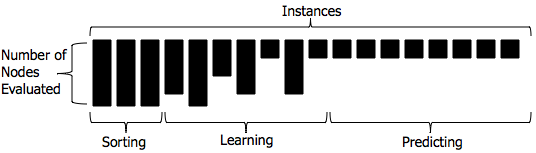
\includegraphics[scale=0.45]{p23.png}
\caption{The number of query nodes that have to be evaluated for every instance is shown. The dynamics of node reduction is illustrated as the process iterates through the instances, from the sorting phase to the learning phase to the prediction phase. Clearly, less queries have to be processed after learning.} 
\label{fig:3phases}
\vspace{-10pt}
\end{figure} 

\textbf{Bounding}. While the branching policy determines the next node to evaluate (and to stop processing one level when the optimal query is found)  the \emph{bounding policy} decides when to stop the whole process. The search should terminate when there exist no or too few matches for the source instances. This can be decided when through many levels, empty candidates sets are obtained as results. In fact, this kind of early termination could also be applied to the search within every level: when too many nodes within the same levels yield empty result, we can move on to the next level. As shown in Alg.~3, the bounding strategy is 
controlled by the parameter $\gamma$. In the experiments in this paper, early termination through bounding is not used because we know in advance that matches exist between the datasets. 
\begin{algorithm}
\caption{CandidateSelection(G, G'). Find candidates for instances in $G$.}
\begin{algorithmic}
\scriptsize\tt
\STATE  sourcekeys  $\leftarrow$ FindKey(G),  targetkey  $\leftarrow$ FindKey(G')
\STATE  keypairs  $\leftarrow$ AligningKeys(sourcekeys, G, targekeys, G') 
\STATE  nodes  $\leftarrow$ BuildNodes(keypairs) 
\STATE  learning  $\leftarrow$ true
\FORALL{b in targetkeys} % Builds a classfier per target key
\STATE predictor[b] $\leftarrow$ NayveBayesClassifier.new()
\ENDFOR 
\FORALL{i in $G$} % Find candidates for each source instance
\IF { $i \geq\gamma$ and candidates = $ \emptyset $ }  %  Validate the bounding policy
\STATE  return null //Satisfied bounding policy
\ENDIF
\FORALL{node in nodes}  
\STATE  b $\leftarrow$ node.targetkey
\IF {cost[b] = 1}  
\STATE next //Satisfied branching policy 
\ENDIF
\IF {learning or predictor[b].predict(node)}  
\STATE  cost[b] = node.evaluate(i) 
\STATE  processed[b] $\leftarrow$  processsed[b] + node 
\IF {learning}  
\STATE    predictor[b].AddExample(node) //Learning Phase
\ENDIF 
\ENDIF 
\ENDFOR
\IF {$i \leq  \beta$} 
\STATE    SortNodesByElapseTime(nodes)  //Sort nodes 
\ENDIF
\IF {test error converges} 
\STATE    learning $\leftarrow$ false
\ENDIF
\IF {$i =ß \alpha$} 
\STATE  examples  $\leftarrow$ matcher(candidates)
\STATE  nodes  $\leftarrow$ updateNodes(examples) 
\STATE    learning $\leftarrow$ true
\ENDIF
\STATE  candidates[i] $\leftarrow$ AggregateMinimalCandidatesSet(processed)
\ENDFOR 
\RETURN candidates[i]
\end{algorithmic}
\end{algorithm}

\textbf{Classifier Prediction}. 
While the branching policy can help to reduce the number of nodes per level, it requires processing all nodes until a query with cardinality 1 is found. This strategy can be further optimized as we observe that given a particular preceding node, the current node to be chosen by the branching strategy mostly has higher cardinality, hence does not need to be executed. To exploit this, we train a classifier, which given a node, predicts if the current node has lower cardinality or not. The process actually include three phases, as illustrated in Fig.~\ref{fig:3phases}. The branch-and-bound strategy is used only in the second and third phase; the predictor only in the third phase. Hence, as evident in Fig.~\ref{fig:3phases}, lesser nodes are executed only in this \emph{Predicting} phase, while there is no or only little reduction of nodes in the first two phases. 

In the \emph{Sorting} phase, nodes are sorted by their average evaluation time. Average time and this order are computed after $\beta \%$ of the instances have been processed. This order is kept to train the classifier and also used during the Prediction phase (so that branching continues with the query that requires lesser time, given they all equal in terms of cardinality). The $\beta$ parameter can be set to be small to obtain average time simply after a few instances (we set it to $1\%$ in the experiment).
 
In the \emph{Learning} phase, the predictor is learned as a Naive Bayes classifier~\cite{Hand2001Idiots}.  It predicts whether the current node to be chosen by the branching strategy indeed has lower cardinality or not. As features, we use the type of the current query, the type of the previous query and a boolean value indicating if the previous query has cardinality greater than zero (i.e. whether it was executed before). 
Recall that the branching policy applies to queries constructed for every key pair and it moves on to next queries when it found an optimal one. Similar to that, a classifier is learned for every set of nodes that share the same target key and accordingly, is only used for queries that have been constructed from this target key. The Learning phase stops soon after three iterations have the same test error. 
When the Learning phase terminates, both the branching policy and the predictor are applied to choose and to skip query nodes, respectively. The effect of branching with and without the predictor is shown in Fig.~\ref{fig:pred}. 

In the \emph{Updating} phase, new template queries are generated with a class clause. The class queries are computed after $\alpha\%$ of the instances have been processed. In this work, we fix $\alpha$ to 5\% of the instances. Then, the candidates obtained so far are input to a matcher that outputs positive and negative examples. As a matcher,  the class-based disambiguator \cite{•} is used in this work, because we assumed the source instances belong to a same class. Those generated examples are input to the algorithm that computes the class clauses. For each class clause found a new query is created by adding it to the original queries. For $q$ queries and $n$ class clauses, then $n \times q$ new queries are generated in the end. After this process, the classifier is retrained using the Leaning procedure described before. 

\begin{figure} 
\vspace{-10pt}
\centering
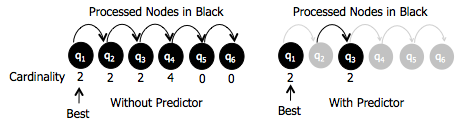
\includegraphics[scale=0.5]{p26.png}
\caption{Nodes are sorted according to cardinality (and time) as discussed, thus first node $q_1$ is chosen by the branching strategy. (Unless a node with cardinality 1 is found), node evaluation sequence without the predictor includes all nodes; with predictor, some nodes may be skipped.} 
\vspace{-10pt}
\label{fig:pred}
\end{figure} 